\documentclass[../main.tex]{subfiles}
\begin{document}
\begin{figure}[h!]
    \centering
    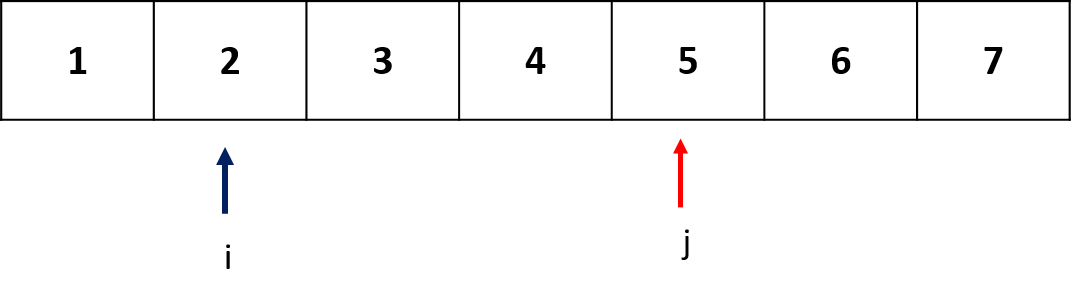
\includegraphics[width=0.7\columnwidth]{fig/two_pointers.png}
    \caption{Two pointer Technique}
    \label{fig:two pointer}
\end{figure}
On linear data structures, or on implicit linear state space, either a particular targeted item or a consecutive substructure such as a subarray and substring can be searched. 

To find a single item on linear space, we can apply linear search in general, or binary search if the data structure is ordered/sorted with logarithmic cost. In this chapter, we introduce two pointer techniques that are commonly used to solve two types of problems:
\begin{enumerate}
    \item Searching: To search for an item such as median,  a predefined substructure, and a substructure that satisfy certain conditions such as finding the minimum subarray length wherein the subarray equals to a targeted sum. Or find a substructure satisfy a string pattern. 
    \item Adjusting: To adjust ordering or arrangement of items in the data structure such as removing duplicates from sorted array. 
\end{enumerate}

% \section{Introduction to Two Pointers}
As the name suggests, Two pointers technique involves two pointers that start and move with the following two patterns:
\begin{enumerate}
    \item Equi-directional:  Both pointers start from the beginning of the array, and usually one moves faster and the other slower. Sliding window algorithm can be put into this category. 
    \item Opposite-directional: One pointer start at the start position and conversely the other pointer starts at the end. These two oppositely posed pointers  move toward each other and usually meet in the middle. 
\end{enumerate}
In the following sections, we will detail on two-pointer technique exemplified on real interview questions.

\section{Slow-Faster Pointers}
Suppose we have two pointers, $i$ and $j$, which may or may not start at the start position in the linear data structures, but one move slower ($i$) and the other faster ($j$). Two pointers can decide either a pair or a subarray to solve related problems.  For the case of subarray, the algorithm is called sliding window algorithm. On the span of the array, and at most of three potential sub-spaces exist: from start index to $i$ ($[0, i]$), from $i$ to $j$ ($[i, j]$), and from $j$ to the end index ($[j, n]$).

Even though slow-faster pointers technique rarely given formal introduction in book, it is widely used in algorithms. In sorting, Lumuto's partition in the QuickSort used the slow-faster pointers to divide the whole region into three parts according the comparison result to the pivot: Smaller Items region, Larger Items region, and the unrestricted region. In string pattern matching, fixed sliding window and one we will introduce in this chapter. 

In this section, we explain how two pointers work on two types of linear data structures: Array and Linked List.
\subsection{Array}
\subsubsection{Remove Duplicates from Sorted Array(L26)} Given a sorted array $a=[0,0,1,1,1,2,2,3,3,4]$, remove the duplicates in-place such that each element appears only once and return the new length. Do not allocate extra space for another array, you must do this by modifying the input array in-place with O(1) extra memory. In the given example, there are in total of 5 unique items and 5 is returned. 
\paragraph{Analysis} We set both slower pointer $i$ and the faster pointer $j$ at the first item in the array. Recall that slow-fast pointers cut the space of the sorted array into three parts, we can define them as:
\begin{enumerate}
    \item unique items in region $[0, i]$,
    \item untouched items in region $[i+1, j]$,
    \item and unprocessed items in region $[j+1, n)$.
\end{enumerate}
In the process, we compare the items pointed by two pointers, once these two items does not equal, we find an new unique item. We copy this unique item at the faster pointer right next to the position of the slower pointer. Afterwards, we move the slow pointer by one position to remove duplicates of our copied value. 


With our example, at first, $i=j=0$, region one has one item which is naively unique and region two has zero item. Part of the process is illustrated as:
\begin{lstlisting}[numbers=none]
i  j   [0, i]  [i+1, j]   process
0  0   [0]     []         item 0==0, j+1=1
0  1   [0]     [0]        item 0==0, j+1=2
0  2   [0]     [0, 1]     item 0!=1, i+1=1, copy 1 to index 1, j+1=3
1  3   [0, 1]  [1, 1]     item 1==1, j+1=4
1  4   [0, 1]  [1, 1, 1]  item 1==1, j+1=5
1  5   [0, 1]  [1, 1, 1, 2]item 1==2, i+1=2, copy 2 to index 2, j+1=6
2  6   [0, 1, 2] [1, 1, 2, 2]
\end{lstlisting}
The code is given as:
\begin{lstlisting}[language=Python]
def removeDuplicates(nums) -> int:
    i, j = 0, 0
    while j < len(nums):
        if nums[i] != nums[j]:
            # Copy j to i+1
            i += 1
            nums[i] = nums[j]
        j += 1
    return i + 1
\end{lstlisting}
After calling the above function on our given example, array $a$ becomes $[[0, 1, 2, 3, 4, 2, 2, 3, 3, 4]$. Check the source code for the whole visualized process.

\subsubsection{Minimum Size Subarray Sum(L209)} Given an array of $n$ positive integers and a positive integer $s$, find the minimal length of a contiguous subarray of which the $sum \geq s$. If there isn't one, return 0 instead.
\begin{lstlisting}[numbers=none]
Example: 

Input: s = 7, nums = [1,4,1,2,4,3]
Output: 2
Explanation: the subarray [4,3] has the minimal length under the problem constraint.
\end{lstlisting}
\paragraph{Analysis} In this problem, we need to secure a substructure--subarray--that not only satisfies a condition($sum \geq s$) but also  has the minimal length. Naively, we can enumerate all subarrays and search through them to find the minimal length, which requires at least $O(n^2)$ time complexity using prefix sum. The code is as:
\begin{lstlisting}[language=Python]
\end{lstlisting}
However, we can use two pointers $i$ and $j$ ($i\leq j)$ and both points at the first item. In this case, these two pointers defines a subarray  $a[i:j+1]$ and we care the region $[i, j]$. As we increase pointer $j$, we keep adding positive item into the sum of the subarray, making the subarray sum monotonically increasing. Oppositely, if we increase pointer $i$, we remove positive item away from the subarray, making the sum of the subarray monotonically decreasing. The detailed steps of two pointer technique in this case is as:
\begin{enumerate}
    \item Get the optimal subarray for all subproblems(subarries) that start from current $i$, which is $0$ at first. We accomplish this by forwarding $j$ pointer to include enough items until $sum \geq s$ that we pause and go to the next step. Let's assume pointer $j$ stops at $e_0$.  
    \item Get the optimal subarray for all subproblems(subarries) that end with current j, which is $e_0$ at the moment. We do this by forwarding pointer $i$ this time to shrink the window size until $sum\geq s$ no longer holds. Let's assume pointer $i$ stops at index $s_0$. Now, we find the optimal solution for subproblems $a[0:i,0:j]$( denoting subarries with the start point in range $[0, i]$ and the end point in range $[0,j]$. 
    \item Now that $i=s_0$ and $j=e_0$, we repeat step 1 and 2.
\end{enumerate}
In our example, we first move $j$ until $j=3$ with a subarray sum of 8. Then we move pointer $i$ until $i=1$ when the subarray sum is less than 7. For subarray $[1, 4, 1, 2]$, we find its optimal solution to have a length 3. The Python code is given as:
\begin{lstlisting}[language=Python]
def minSubArrayLen(s: int, nums) -> int:
    i, j = 0, 0
    acc = 0
    ans = float('inf')
    while j < len(nums):
        acc += nums[j]
        # Shrink the window
        while acc >= s:
            ans = min(ans, j - i + 1)
            acc -= nums[i]
            i += 1
        j += 1
        
    return ans if ans < float('inf') else 0
\end{lstlisting}

Because both pointer $i$ and $j$  move at most $n$ steps, with the total operations to be at most $2n$, making the time complexity as $O(n)$. The above question would be trivial if the maximum subarray length is asked.

\subsection{Minimum Window Substring (L76, hard)} 
 Given a string $S$ and a string $T$, find all the minimum windows in $S$ which will contain all the characters in $T$ in complexity $O(n)$.
\begin{lstlisting}[numbers=none]
Example:
Input: S = "AOBECDBANC", T = "ABC"
Output: ["CDBA", "BANC"]
\end{lstlisting}
\begin{figure}[h!]
    \centering
    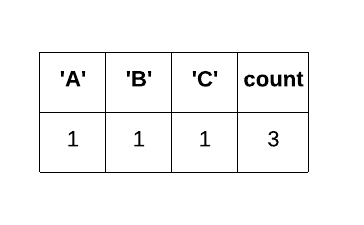
\includegraphics[width=0.5\columnwidth]{fig/minimum_window_substring.png}
    \caption{The data structures to track the state of window.}
    \label{fig:minimum_window}
\end{figure}
\paragraph{Analysis} Applying two pointers, with the region between pointer $i$ and $j$ to be our testing substring. For this problem, the condition for the window $[i, j]$ it will at most have all characters from $T$. The intuition is we keep expanding the window by moving forward $j$ until all characters in $T$ is found. Afterwards, we contract the window so that we can find the minimum window with the condition satisfied. Instead of using another data structure to track the state of the current window, we can depict the pattern $T$ as a dictionary data structure where all unique characters comprising the keys and with the number of occurrence of each character as value. We use another variable \texttt{count} to track how the number of unique characters. In all, they are used to track the state of the moving window in $[i, j]$, with the value of the dictionary to indicate how many occurrence is short of, and the \texttt{count} represents how many unique characters is not fully found, and we depict the state  in Fig.~\ref{fig:minimum_window}. 

\begin{figure}[h!]
    \centering
    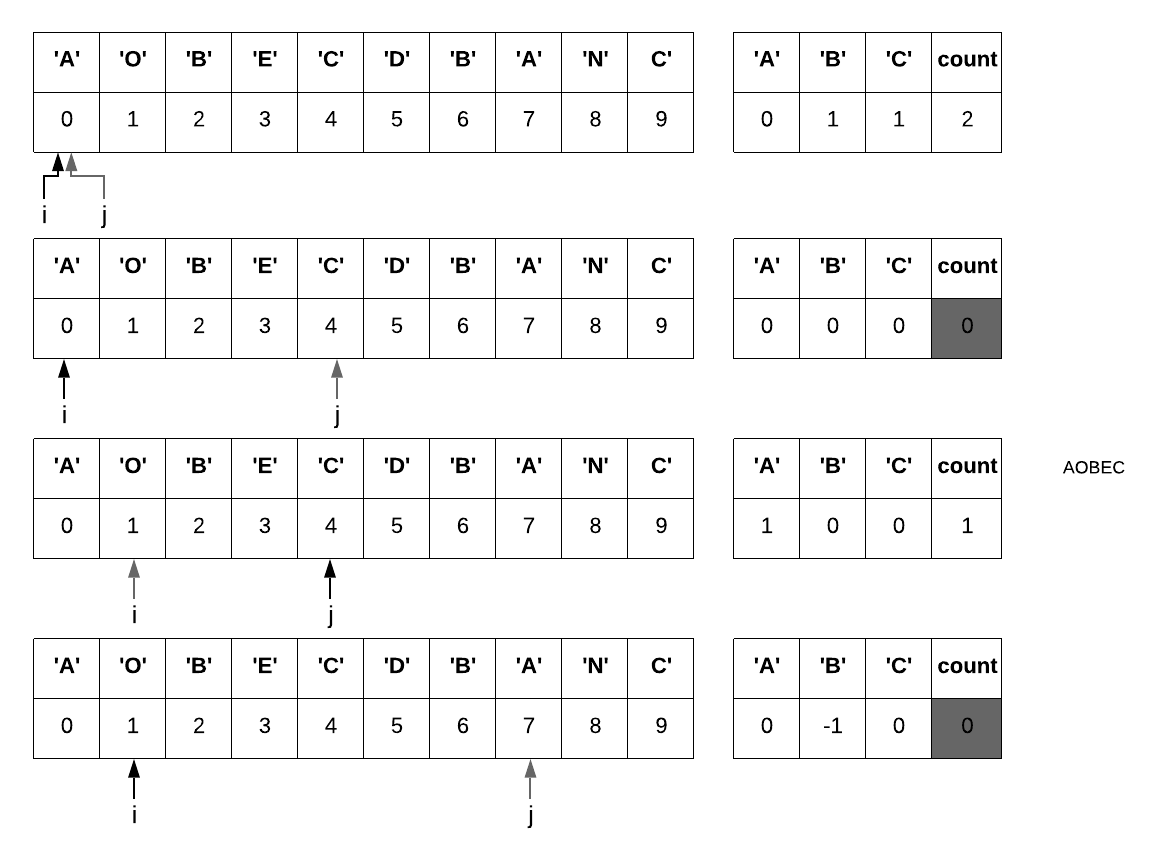
\includegraphics[width=1.1\columnwidth]{fig/minimum_window_substring_process.png}
    \caption{The partial process of applying two pointers. The grey shaded arrow indicates the pointer that is on move.}
    \label{fig:minimum_window_process}
\end{figure}

Along the expanding and shrinking of the window that comes with the movement of pointer $i$ and $j$, we track the state with:
\begin{itemize}
    \item When forwarding $j$, we encompass $S[j]$ in the window. If $S[j]$ is a key in the dictionary, decrease the value by one. Further, if the value reaches to the threshold $0$, we decrease \texttt{count} by one, meaning we are short of one less character in the window.
    \item Once \texttt{count=0}, our window satisfy condition for contracting. We then forward $i$, removing $S[i]$ from the window if it is existing key in the dictionary by increasing this key's value, meaning the window is short of one more character. Once the value reaches to the threshold of $1$, we increase $count$. 
\end{itemize}
Part of this process with our example is shown in Fig.~\ref{fig:minimum_window_process}. And the Python code is given as:
\begin{lstlisting}[language=Python]
from collections import Counter
def minWindow(s, t):
  dict_t = Counter(t)
  count = len(dict_t)
  i, j = 0, 0
  ans = []
  minLen = float('inf')
  while j < len(s):
    c = s[j]
    if c in dict_t:
      dict_t[c] -= 1
      if dict_t[c] == 0:
        count -= 1
    # Shrink the window
    while count == 0 and i < j:
      curLen = j - i + 1
      if curLen < minLen:
        minLen = j - i + 1
        ans = [s[i:j+1]]
      elif curLen == minLen: 
        ans.append(s[i:j+1])

      c = s[i]
      if c in dict_t:
        dict_t[c] += 1
        if dict_t[c] == 1:
          count += 1
      i += 1

    j += 1
  return ans
\end{lstlisting}

% until When the window has all the desired characters, we contract (if possible) and save the smallest window till now. The only difference compared with the above problem is the definition of desirable: we need to compare the state of current window with the required state in T. They can be handled as a hashmap with character as key and frequency of characters as value. 
% \begin{lstlisting}[language=Python]
% def minWindow(self, s, t):
%     dict_t = Counter(t)
%     state = Counter()
%     required = len(dict_t)

%     # left and right pointer
%     i, j = 0, 0

%     formed = 0
%     ans = float("inf"), None # min len, and start pos

%     while j < len(s):
%         char = s[j]
%         # record current state
%         if char in dict_t:
%             state[char] += 1
%             if state[char] == dict_t[char]:
%                 formed += 1

%         # Try and contract the window till the point where it ceases to be 'desirable'.
%         # bPrint = False
%         while i<=j and formed == required:
%             # if not bPrint:
%             #     print('found:', s[i:j+1], i, j)
%             #     bPrint = True
%             char = s[i]
%             if j-i+1 < ans[0]:
%                 ans = j - i + 1, i
%             # change the state
%             if char in dict_t:
%                 state[char] -= 1
%                 if state[char] == dict_t[char]-1:
%                     formed -= 1

%             # Move the left pointer ahead,
%             i += 1    
        
%         # Keep expanding the window 
%         j += 1  
%         # if bPrint:
%         #     print('move to:', s[i:j+1], i, j)
%     return "" if ans[0] == float("inf") else s[ans[1] : ans[1] + ans[0]]
% \end{lstlisting}

% The process would be:
% \begin{lstlisting}[numbers=none]
% found: ADOBEC 0 5
% move to: DOBECO 1 6
% found: DOBECODEBA 1 10
% move to: ODEBAN 6 11
% found: ODEBANC 6 12
% move to: ANC 10 13
% \end{lstlisting}
\subsection{When Two Pointers do not work} Two pointer does not always work on subarray related problems.
\begin{bclogo}[couleur = blue!30, arrondi=0.1,logo=\bccrayon,ombre=true]{What happens if there exists negative number in the array? } Since the sum of the subarray is no longer monotonically increasing with the number of items between two pointers, we can not figure out how to move two pointers each step. Instead (1) we can use prefix sum and organize them in order, and use binary search to find all possible start index.  (2) use monotone stack (see  LeetCode probelm: 325. Maximum Size Subarray Sum Equals k, 325. Maximum Size Subarray Sum Equals k (hard)))
\end{bclogo}

\begin{bclogo}[couleur = blue!30, arrondi=0.1,logo=\bccrayon,ombre=true]{What if we are to check the maximum average subarray? } 
644. Maximum Average Subarray II (hard). Similarly, the average of subarray does not follow a certain order with the moving of two pointers at each side, making it impossible to decide how to make the two pointers.

\end{bclogo}

\subsection{Linked List}
The complete code to remove cycle is provided in google colab together with running examples.
\subsubsection{Middle of the Linked List(L876)} 
%The simplest example of slow-fast pointers on linked list is to get the middle node of a given linked list. 
Given a non-empty, singly linked list with head node $head$, return a middle node of linked list. When the linked list is of odd length, there exists one and only middle node, but when it is of even length, two exists and we return the second middle node.
\begin{lstlisting}[numbers=none]
Example 1 (odd length):

Input: [1,2,3,4,5]
Output: Node 3 from this list (Serialization: [3,4,5])

Example 2 (even length):

Input: [1,2,3,4,5,6]
Output: Node 4

 from this list (Serialization: [4,5,6])
\end{lstlisting}

\paragraph{Analysis} If the data structure is array, we can compute the position of the middle item simply with the total length. Following this method, if only one pointer is applied, we can first iterate over the whole linked list in $O(n)$ time to get the length. Then we do another iteration to obtain the middle node. $n + \frac{n}{2}$ times of operations  needed, making the time complexity $O(n)$. 

However, we can apply two pointers simultaneously at the head node, each one moves at different paces: the slow pointer moves one step at a time and the fast moves two steps instead. When the fast pointer reached the end, the slow pointer will stop at the middle. This slow-faster pointers technique requires only $\frac{n}{2}$ times of operations, which is three times faster than our naive method, although the big Oh time complexity still remains $O(n)$. 
\paragraph{Implementation}
\begin{figure}[h]
    \centering
    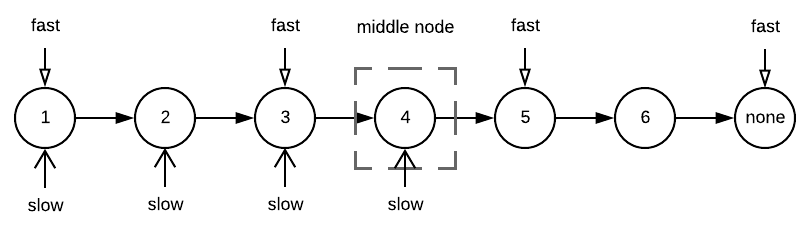
\includegraphics[width = 0.98\columnwidth]{fig/middle_of_linked_list.png}
    \caption{Slow-fast pointer to find middle}
    \label{fig:slow-faster}
\end{figure}
Simply, we  illustrate the process of running the two pointers technique on our two examples in Fig.~\ref{fig:slow-faster}. As we can see, when the slow pointer reaches to item 3, the faster pointer is at item 5, which is the last item in the first example that comes with odd length. Further, when the slow pointer reaches to item 4, the faster pointer reaches to the empty node of the last item in the second example that comes with even length. Therefore, in the implementation, we check two conditions in the \texttt{while} loop: 
\begin{enumerate}
    \item For example 1: if the fast pointer has no successor (\texttt{fast.next==None}), the loop terminates.
    \item For example 1: if the fast pointer is invalid (\texttt{fast==None}), the loop terminates.
\end{enumerate}
The Python code is as:
\begin{lstlisting}[language=Python]
def middleNode(head):
    slow = fast = head
    while fast and fast.next:        
        fast = fast.next.next
        slow = slow.next     
    return slow
\end{lstlisting}

\subsubsection{Floyd's Cycle Detection (Floyd's Tortoise and Hare)} 
\begin{figure}[h!]
    \centering
    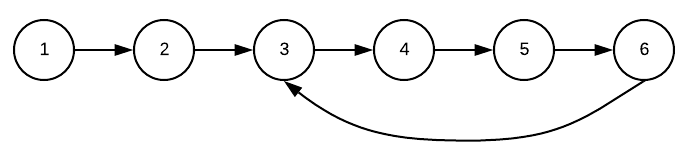
\includegraphics[width=0.8\columnwidth]{fig/circular_linked_list.png}
    \caption{Circular Linked List}
    \label{fig:circular_linked_list}
\end{figure}
When a linked list which has a cycle, as shown in Fig.~\ref{fig:circular_linked_list}, iterating items over the list will make the program stuck into infinite loop. The pointer starts from the heap, traverse to the start of the loop, and then comes back to the start of the loop again and continues this process endlessly. To avoid being stuck into a ``trap'', we have to possibly solve the following three problems:
\begin{enumerate}
    \item Check if there exists a cycle. 
    \item Check where the cycle starts.
    \item Remove the cycle once it is detected.
\end{enumerate}
The solution encompasses the exact way of slow faster pointers traversing through the linked list as our last example. With the slow pointer iterating one item at a time, and the faster pointer in double pace, these two pointers will definitely meet at one item in the loop. In our example, they will meet at node 6. So, is it possible that it will meet at the non-loop region starts from the heap and ends at the start node of the loop? The answer is No, because the faster pointer will only traverse through the non-loop region once and it is always faster than the slow pointer, making it impossible to meet in this region.  This method is called Floyd's Cycle Detection, aka Floyd's Tortoise and Hare Cycle Detection. Let's see more details at how to solve our mentioned three problems with this method. 
\paragraph{Check Linked List Cycle(L141)}
Compared with the code in the last example, we only need to check if the \texttt{slow} and \texttt{fat} pointers are pointing at the same node: If it is, we are certain that there must be a loop in the list and return \texttt{True}, otherwise  return \texttt{False}.
\begin{lstlisting}[language=Python]
def hasCycle(head):
    slow = fast = head
    while fast and fast.next:
        slow = slow.next
        fast = fast.next.next
        if slow == fast:
            return True
    return False
\end{lstlisting}
\paragraph{Check Start Node of Linked List Cycle(L142)} Given a linked list, return the node where the cycle begins. If there is no cycle, return \texttt{None}.
\begin{figure}[h!]
    \centering
    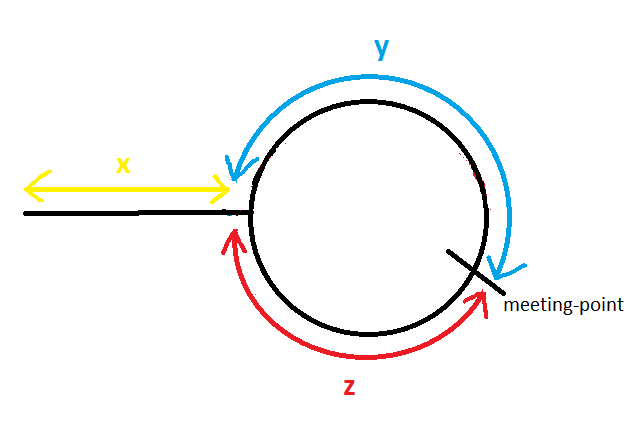
\includegraphics[width=0.6\columnwidth]{fig/TQoyH.png}
    \caption{Floyd's Cycle finding Algorithm}
    \label{fig:floyd_cycle_1}
\end{figure}

For a given linked list, assume the slow and fast pointers meet at node somewhere in the cycle. As shown in Fig.~\ref{fig:floyd_cycle_1}, we denote  three nodes: head ($h$, start node of cycle($s$), and meeting node in the cycle($m$). we denote the distance between $h$ and $s$ to be $x$, the distance between $s$ and $m$ to be $y$, and the distance between $m$ and $s$ to be $z$.  Because the faster pointer traverses through the list in double speed, when it meets up with the slow pointer, the distance that it traveled($x+y+z+y$) to be two times of the distance traveled by the slow pointer ($x+y$).
\begin{align}
    x + y + z + y &= x + y \\
    x = z
\end{align}
From the above equation, we obtain the equal relation between $x$ and $z$. the starting node of the cycle from the head is $x$, and $y$ is the distance from the start node to the slow and fast pointer's node, and $z$ is the remaining distance from the meeting point to the start node.  Therefore, after we have detected the cycle from the last example, we can reset the slow pointer to the head of the linked list after. Then we make the slow and the fast pointer both traverse at the same pace--one node at a time--until they meet at a node we stop the traversal. The node where they stop at is the start node of the cycle. The code is given as:

% the meeting point, and making both slow and fast pointer to move one node at a time, they will meet at the starting node of the cycle.


% Now, let's try to device the algorithm. Both slow and fast pointer starts at position 0, the node index they travel each step is: [0,1,2,3,...,k] and [0,2,4,6,...,2k] for slow and fast pointer respectively. Therefore, the total distance traveled by the slow pointer is half of the distance travelled by the fat pointer. From the above figure, we have the distance travelled by slow pointer to be $d_s = x+y$, and for the fast pointer $d_f = x+y+z+y = x+2y+z$. With the relation $2*d_s = d_f$. We will eventually get $x = z$. Therefore, by moving slow pointer to the start of the linked list after the meeting point, and making both slow and fast pointer to move one node at a time, they will meet at the starting node of the cycle. (LeetCode problem: 142. Linked List Cycle II (medium)).
\begin{lstlisting}[language=Python]
def detectCycle(head):
    slow = fast = head

    def getStartNode(slow, fast, head):
      # Reset slow pointer      
      slow = head
      while fast and slow != fast:
          slow = slow.next
          fast = fast.next
      return slow

    while fast and fast.next:
        slow = slow.next
        fast = fast.next.next
        # A cycle is detected
        if slow == fast: 
            return getStartNode(slow, fast, head)
    
    return None
\end{lstlisting}

\paragraph{Remove Linked List Cycle}
We can remove the cycle by recirculing the last node in the cycle, which in example in Fig.~\ref{fig:circular_linked_list} is node 6 to an empty node. Therefore, we have to modify the above code to make the \texttt{slow} and {fast} pointers stop at the last node instead of the start node of the loop. This subroutine is implemented as:
\begin{lstlisting}[language=Python]
def resetLastNode(slow, fast, head):
    slow = head
    while fast and slow.next != fast.next:
        slow = slow.next
        fast = fast.next
    fast.next = None
\end{lstlisting}
The complete code to remove cycle is provided in google colab together with running examples.
\begin{bclogo}[couleur = blue!30, arrondi=0.1,logo=\bccrayon,ombre=true]{What if there has not only one, but multiple cycles in the Linked List? } 
\end{bclogo}

\section{Opposite-directional Pointers}
Another variant of two pointers technique is to place these two pointers oppositely: one at the beginning and the other at the end of the array. Through the process, they move toward each other  until they meet in the middle. Details such as how much each pointer moves or which pointer to move at each step decided by our specific problems to solve. We just have to make sure when we are applying this technique, we have considered its whole state space, and will not miss out some area which makes the search incomplete. 

The simplest example of this two pointers method is to reverse an array or a string around. For example, when the list $a=[1, 2, 3, 4, 5]$ is reversed, it becomes $[5, 4, 3, 2, 1]$. Of course we can simply assign a new list and copy the items in reversed orders. But, with two pointers, we are able to reverse it in-place and using only $O(\frac{n}{2})$ times of operations through the following code:
\begin{lstlisting}[language=Python]
def reverse(a):
  i, j = 0, len(a) - 1
  while i < j:
    # Swap items
    a[i], a[j] = a[j], a[i]
    i += 1
    j -= 1
\end{lstlisting}
Moreover, binary search can be viewed as an example of opposite-directional pointers. At first, these two pointers are the first and the last item in the array. Then depends on which side of the target compared with the item in the middle, one of the pointers move either forward or backward to the middle point, reducing the search space to half of where it started at each step.  We also explore another example with this technique.
\subsubsection{Two Sum on Sorted Array(L167)} 
Given an array of integers that is already sorted in ascending order, find two numbers such that they add up to a specific target number. 
\begin{lstlisting}[numbers=none]
Input: numbers = [2,7,11,15], target = 9
Output: [1,2]
Explanation: The sum of 2 and 7 is 9. Therefore index1 = 0, index2 = 1.
\end{lstlisting}
\paragraph{Analysis} If we simply put enumerate all possible pairs, we have to take $O(n^2)$ to solve this problem. However, with the opposite-directional two pointers, it gives out linear performance.

Denote the list as $A=[a_1, a_2, ..., a_{n-1}, a_{n}]$, and for the sorted array we have $a_1\leq a_2 \leq...\leq  a_{n-1} \leq a_n$. The range of the sum of any two items in the array is within two possible ranges: $[a_1+a_2, a_1+a_n]$ and $[a_1+a_n, a_{n-1}+a_n]$.  By placing one pointer $i$ at $a_1$ and the other $j$ at $a_n$ to start with, we can get $a_1+a_n$ as the sum. Pointer $i$ can only move forward, accessing larger items. On the other hand, pointer $j$ can only backward, accessing smaller items. Now there are three scenarios according to the comparison between the target and the current sum of the two pointers:
\begin{enumerate}
    \item  If $t == a[i] + a[j]$, target sum found.
    \item  If $t > a[i] + a[j]$, we have to increase the sum, we can only do this by moving pointer $i$ forward.
    \item If $t > a[i] + a[j]$, we have to decrease the sum, we can only do this by moving pointer $j$ backward.
\end{enumerate}
The Python code is as:
\begin{lstlisting}[language=Python]
def twoSum(a, target):
    n = len(a)
    i, j  = 0, n-1
    while i < j:
        temp = a[i] + a[j]
        if temp == target:
            return [i, j]
        elif temp < target:
            i += 1
        else:
            j -= 1
    return []
\end{lstlisting}
\section{Follow Up: Three Pointers}
Sometimes, manipulating two pointers is not even enough to distinguish different subspaces, we might need to the assistant of one another pointer to make things  work.
\subsubsection{Binary Subarrays With Sum (L930)} In an array $A$ of $0$s and $1$s, how many non-empty subarrays have sum $S$?
\begin{lstlisting}[numbers=none]
Example 1:
Input: A = [1,0,1,0,1], S = 2
Output: 4
Explanation: 
The 4 subarrays are listed below:
[1,0,1], index (0, 2)
[1,0,1,0], index (0, 3)
[0,1,0,1], index (1, 4)
[1,0,1], index (2, 4)
\end{lstlisting}
\paragraph{Analysis}
This problem is highly similar to the minimum length subarray problem we encountered before. We naturally start with two pointers $i$ and $j$, and restrict the subarray in range $[i, j]$ to satisfy condition $sum\leq S$. The window is contracted when the condition is violated. We would have write the following code:
\begin{lstlisting}[language=Python]
def numSubarraysWithSum(a, S):
  i, j = 0, 0
  win_sum = 0
  ans = 0
  while j < len(a):
    win_sum += a[j]
    while i < j and win_sum > S:
      win_sum -= a[i]
      i += 1
    if win_sum == S:
      ans += 1
      print('({}, {})'.format(i, j))
    j += 1
  return ans
\end{lstlisting}
However, the above code only returns $3$, instead of $4$ as shown in the example. By printing out pointers $i$ and $j$, we can see the above code is missing case $(2, 4)$. Why? Because we are restricting the subarray sum in range $[i, j]$ to be smaller than or equal to $S$, with the occruence of $0$s that might appear in the front or in the rear of the subarray:
\begin{itemize}
\item In the process of expanding the subarray, pointer $j$ is moved one at a time. Thus, even though $0$s appear in the rear of the subarray, the counting is correct.
\item However, in the process of shrinking the subarray while the restriction is violated($sum > S$), we stop right away once $sum \leq S$. And in the code, we end up only counting it as one occurrence. With $0$s at the beginning of the subarray, such as the subarray $[0, 1, 0, 1]$ with index $1$ and $4$, there count should be two instead of one. 
\end{itemize}
The solution is to add another pointer $i_h$ to handle the missed case: When the $sum=S$, count the total occurrence of $0$ in the front. Compared with the above solution, the code only differs slightly with the additional pointer and one extra \texttt{while} loop to deal the case. Also we need to pay attention that $i_h \leq j$, otherwise, the \texttt{while} loop would fail with example with only zeros and a targeting sum $0$.
\begin{lstlisting}[language=Python]
def numSubarraysWithSum(a, S):
  i, i_h, j = 0, 0, 0
  win_sum = 0
  ans = 0
  while j < len(a):
    win_sum += a[j]
    while i < j and win_sum > S:
      win_sum -= a[i]
      i += 1
    # Move i_h to count all zeros in the front
    i_h = i
    while i_h < j and win_sum == S and a[i_h] == 0:
      ans += 1
      i_h += 1
      
    if win_sum == S:
      ans += 1
    j += 1
  return ans
\end{lstlisting}

We noticed that in this case, we have to explicitly restrict $i < j$ and $i_h < j$ due to the special case,  while in all our previous examples, we do not have to.

\section{Summary}
Two pointers is a powerful tool for solving problems on liner data structures, such as ``certain'' subarray and substring problems as we have shown in the examples. The ``window'' secluded between the two pointers can be viewed as sliding window: It can move slide forwarding with the forwarding the slower pointer. Two important properties are generally required for this technique to work:
\begin{enumerate}
\begin{figure}[h!]
    \centering
    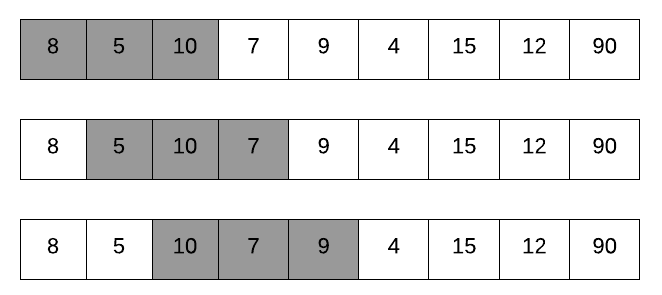
\includegraphics[width=0.7\columnwidth]{fig/Sliding_window_property.png}
    \caption{Sliding Window Property}
    \label{fig:slide_window}
\end{figure}
    \item Sliding window property: Either we move the faster pointer $j$ forward by one, or move the slower pointer $i$, we can get the state of current window in $O(1)$ cost knowing the state of the last window. 
    
    For example, given an array, imagine that we have a fixed size window as shown in Fig.~\ref{fig:slide_window}, and we can slide it forward one position at a time, compute the sum of each window. The bruteforce solution would be of $O(kn)$ complexity where $k$ is the window size and $n$ is the array size by using two nested \texttt{for} loops: one to set the starting point, and the other to compute the sum in $O(k)$. However, the sum of the current window ($S_c$) can be computed from the last window ($S_l$), and  the items that just slid out and in as $a_j$ and $a_i$ respectively. Then $S_c = S_l-a_i+a_j$. Getting the state of of the window between two pointers in $O(1)$ as shown in the example is our called Sliding Window Property.
    
    Usually, for an array with numerical value, it satisfies the sliding window property if we are to compute its sum or product. For substring, as shown in our minimum window substring example, we can get the state of current window referring to the state of the last window in $O(1)$ with the assist of dictionary data structure. In substring, this is more obscure, and the general requirement is that the state of the substring does not relate to the order of the characters(anagram-like state). 
    
    \item Monotonicity: For subarray sum/product, the array should only comprise all positive/negative values so that the prefix sum/product has monotonicity: moving the faster pointer and the slower pointer forward results into opposite change to the state.  The same goes for the substring problems where we see from the minimum window substring example the change of the state: \texttt{count} and the value of the dictionary is monotonic, and each either increases or decreases with the moving of two pointers.
% \begin{lstlisting}[language=Python]
% def fixedSlideWindow(A, k):
%     n = len(A)
%     if k >= n:
%         return sum(A)
%     # compute the first window
%     acc = sum(A[:k])
%     ans = acc
%     # slide the window
%     for i in range(n-k): # i is the start point of the window
%         j = i + k # j is the end point of the window
%         acc = acc - A[i] + A[j]
%         ans = max(ans, acc)
%     return ans
% \end{lstlisting}
\end{enumerate}

% The steps of using sliding windows:
% \begin{enumerate}
%     \item Initialize the left and right pointer;
%     \item Handle the right pointer and record the state of the current window;
%     \item While the window is in the state of desirable: record the optimal solution, move the left pointer and record the state (change or stay unchanged).
%     \item Up till here, the state is not desirable.  Move the right pointer in order to find a desirable window;
% \end{enumerate}
\section{Exercises}
\begin{enumerate}
\item 3. Longest Substring Without Repeating Characters
\item 674. Longest Continuous Increasing Subsequence (easy)
\item 438. Find All Anagrams in a String
\item 30. Substring with Concatenation of All Words
\item 159. Longest Substring with At Most Two Distinct Characters
\item 567. Permutation in String
\item 340. Longest Substring with At Most K Distinct Characters
\item 424. Longest Repeating Character Replacement
\end{enumerate}
% that data strArray Search is to find a \textbf{sub-structure} on a given linear data structure( Chapter~\ref{chapter_linear_data_structure}) or a virtual linear search space. Categorized by the definition of sub-structure:
% \begin{itemize}
%     \item Define the sub-structure as a \textbf{particular item}: Usually the worst and average performance is $O(n)$.  \textbf{Binary search} (Section~\ref{sec_binary_search}) finds an item within an ordered data structure, each time, the search space is elimilated by half in size, which makes the worst time complexity $O(\log n)$. Using hashmap can gain us the best complexity of $O(1)$. 
%     \item Define the sub-structure as a \textbf{consecutive substructure} indexed by a start and end index (subarray) in the linear data structure, we introduce the \textbf{Sliding Window Algorithm} (Section~\ref{sec_pointer_sliding_window}). Compared with the brute force solution, it decrease the complexity from $O(n^2)$ to $O(n)$. If the sub-structure is \textbf{predefined pattern}, we need pattern matching algorithms. This usually exists in string data structure, and we do string pattern matching (Section~\ref{}). 
% \end{itemize}

% \subfile{chapters/learning/search/sliding_window}






 \end{document}